% Various updates/fixes - CLM, June-2008)
%
\section{Interpolation / Extrapolation Tool\label{interpolation}}

It is often desirable to predict performance of non-existent machines, or across architectures.
This section describes a  tool that rewrites the  log files produced by BigSim (also known as {\em bgTrace trace
logs}) to provide new durations for portions of the application consisting of sequential execution blocks.
These new durations can be based upon multiple types of models.
The tool can be easily modified to add new types of models if the user requires.
The models can be generated from full or partial executions of an application on an existing processor or on a
cycle-accurate simulator. 


When predicting the runtime of a parallel application on a not-yet-existent
parallel platform, there are two important concerns. The first is correctly modeling the
interconnection network, which is handled by BigSimulator (also called BigNetSim). 
The second is determining the durations of the relevant sequential portions of code,
which we call \textbf{Sequential Execution Blocks (SEB)}, on a new type of processor.
The interpolation tool of this section handles only the prediction of SEB durations,
using currently three types of implemented models:

\begin{enumerate}
\item \textbf{Scaling of SEB durations} observed on an available (existing) processor, via multiplcation of
the original durations by a constant factor.
\item \textbf{Parameterizations of SEBs}: each SEB is augmented with user-defined parameters that
influence the duration of the SEB. An extrapolation model based on those parameters can
predict the durations of SEBs not instrumented in the initial emulation run.
\item \textbf{Parameterizations with cycle-accurate simulations} for non-existent architectures: 
processor designers use cycle-accurate simulators to simulate the performance of a piece of code on
a future processor that is currently unavailable.  Timings for each SEB can be estimated in such a cycle-accurate
simulator. The cycle-accurate timings can be extrapolated to predict the durations of SEBs not instrumented in the
cycle-accurate simulator.
\end{enumerate}

This tool will soon include a new model with support for performance counters.
The currently available tool rewrites the log files produced by a run in the BigSim Emulator. 
The rewritten log files can then be consumed by BigSimulator. This usage flow can be seen in
Figure~\ref{fig:interpolationflow}, showing that multiple types of models are supported in the tool. 

\begin{figure}[!t]
\centering  
  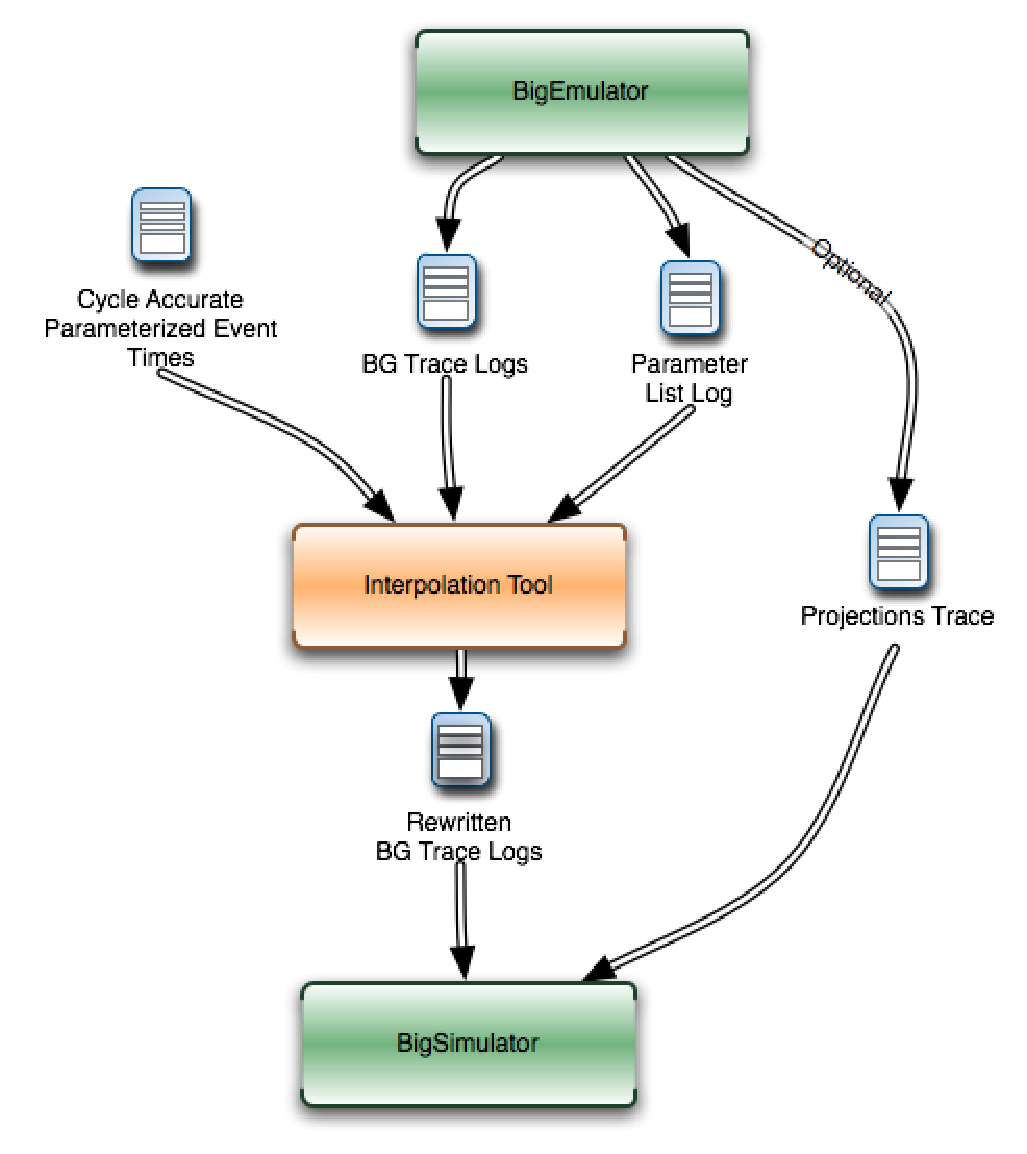
\includegraphics[width=4in]{figures/InterpolationFlow}
{\sffamily\bfseries\small \caption{Flow diagram for use of the interpolation tool\label{fig:interpolationflow}}}
\end{figure}

%%%%%%%%%%%%%%%%%%%%%%%%%%%%%%%%%%%%%%%%%%%%%%%%%%%%
\subsection{Usage\label{usage}}

The interpolation tool is part of the regular \charmpp{} distribution and 
can be found under the directory \texttt{charm/examples/bigsim/tools/rewritelog} with a \texttt{README} file describing its use in more detail than this manual.

\subsubsection{Producing the Parameterized Timings Log}
The interpolation tool uses as input a log of actual durations of user-bracketed sequential execution blocks.
These timings come from a full or partial execution of the parallel application on a real machine or
within a cycle-accurate simulator. 

The user must insert \texttt{startTraceBigSim()} and  \texttt{endTraceBigSim()} calls around the main
computational regions in the parallel application. These two calls bracket the region of interest
and print out a record for that computational region. The functions should be called at most once during
any SEB. The output produced by  \texttt{endTraceBigSim()} is a line similar to

 ``\texttt{TRACEBIGSIM: event:\{ PairCalculator::bwMultiplyHelper \}  time:\{ 0.002586 \}  params:\{ 16384.00 1.00 220.00 128.00 128.00 0.00 0.00 0.00 \}}.'' 

\noindent
The event name and the values (in double-precision floating-point) for up to 20 parameters are
specified in the call to  \texttt{endTraceBigSim()}; the \texttt{time} field records  the duration of the bracketed region of sequential code. 

To run in a cycle-accurate simulator such as IBM's MAMBO, the  \texttt{startTraceBigSim()} and  \texttt{endTraceBigSim()} functions would be modified to switch between the ``fast forward'' mode used during the rest of the
program and the cycle-accurate mode during the bracketed region of code. The functions are provided in C++ source files under the directory \texttt{charm/examples/bigsim/tools/rewritelog/traceBigSim} and their calls
must be added to an application's source file manually.

%%%%%%%%%%%%%%%%%%%%%%%%%%%%%%%%%%%%%%%%%%%%%%%%%%%%
\subsubsection{The BigSim log file format}

To understand how the interpolation tool works, it is instructive to consider the format
of logs produced by the BigSim Emulator.
A BigSim log file (i.e. bgTrace log) contains data from emulation of the full parallel application.
There is an entry for each SEB, with the following fields:  \textit{ID}, \textit{Name}, $T_{start}$,
$T_{end}$, \textit{Back}, \textit{Forward}, \textit{Message ID}, \textit{Source Node},
\textit{Message ID}, \textit{Sent Messages}. The final field is actually a list of records for each
message sent by the execution block; each record contains the following fields:
 \textit{Message ID}, $T_{sent}$, $T_{recv}$, \textit{Destination PE}, \textit{Size}, \textit{Group}.

The interpolation tool will rewrite the durations of the SEBs by correcting the $T_{end}$ field for the
SEB and the $T_{sent}$ fields for each message sent. The new durations of all SEBs will be based upon
some model $M:SEB\rightarrow Duration$. 

Each SEB can be decomposed into three temporal regions as shown in Figure~\ref{event_diagram}. 
The entire SEB is associated with execution of a Charm++ entry method, while the middle region
is the computational kernel of interest, bracketed by the user's \texttt{startTraceBigSim()} and  \texttt{endTraceBigSim()} calls. The model is used only to approximate the new duration of the middle temporal region;
the durations of the beginning and ending regions are simply scaled by a constant factor.
Internally, the interpolation tool takes the ID for each SEB and looks up its associated parameters.
%If
When those parameters are found, they are used as input for evaluation of the new duration $d_{new}$
for the SEB. The end time is then modified to be $T_{end}\leftarrow  T_{start}+d_{new}$.

\begin{figure}
\centering
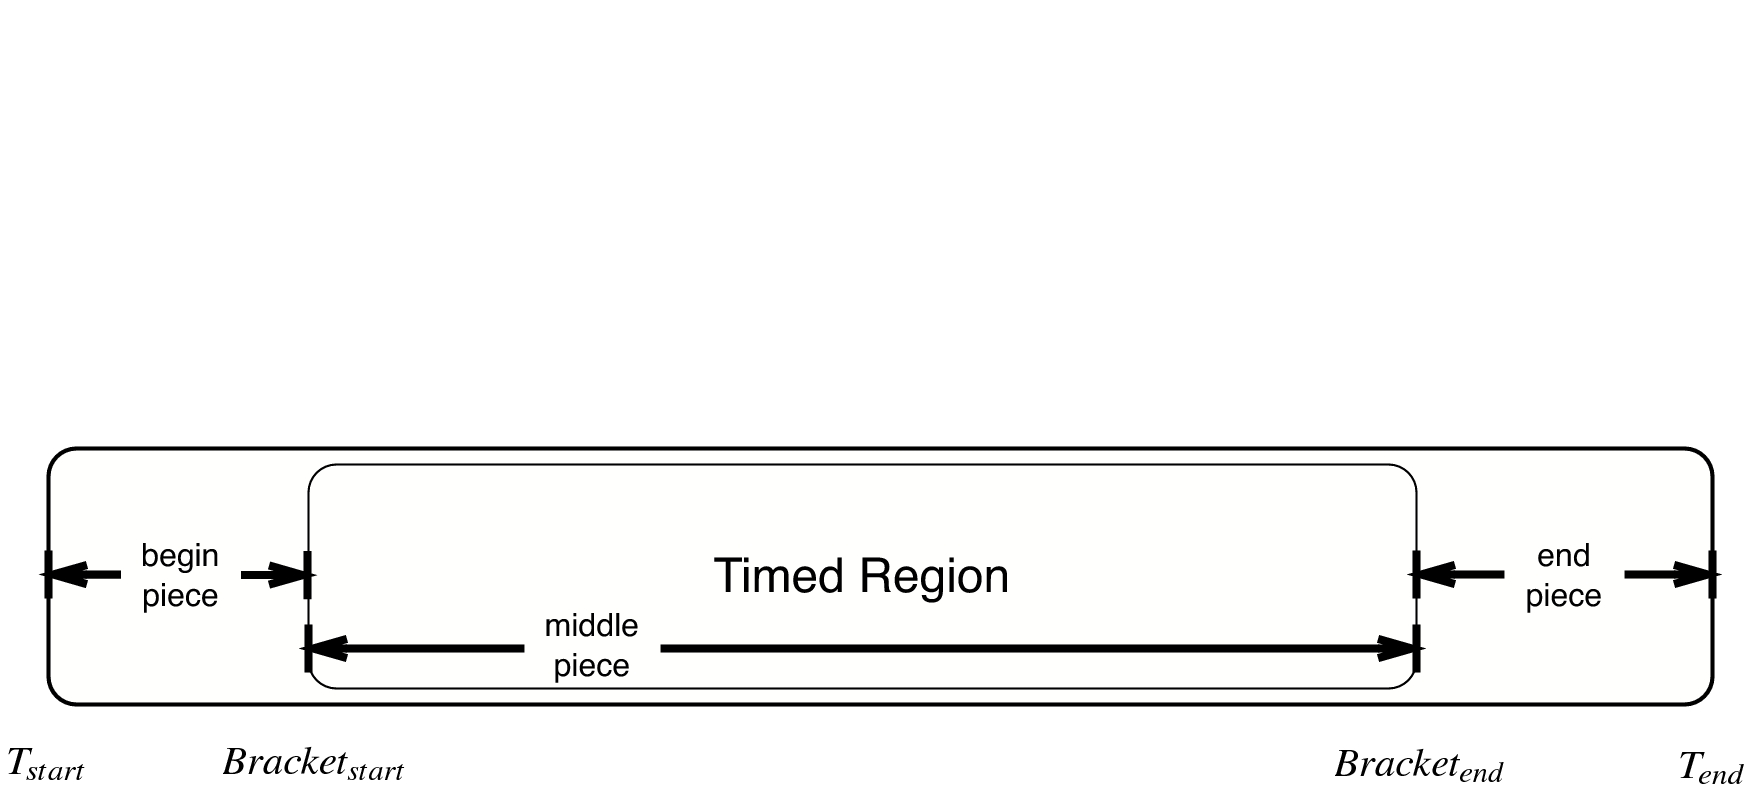
\includegraphics[width=5in]{figures/event_diagram}
\caption{SEBs in the bgTrace file have a start and end time. Only a portion of the SEB, e.g. the important compuational kernel, is timed when performing cycle accurate simulation. The duration of the middle portion of the SEB can be estimated in a different manner than the rest of the SEB. For example, the begin and end pieces can be scaled by some constant factor, while the bracketed middle region's duration can be estimated based on a more
sophisticated model.
\label{event_diagram}}
\end{figure}

\begin{figure}
\centering
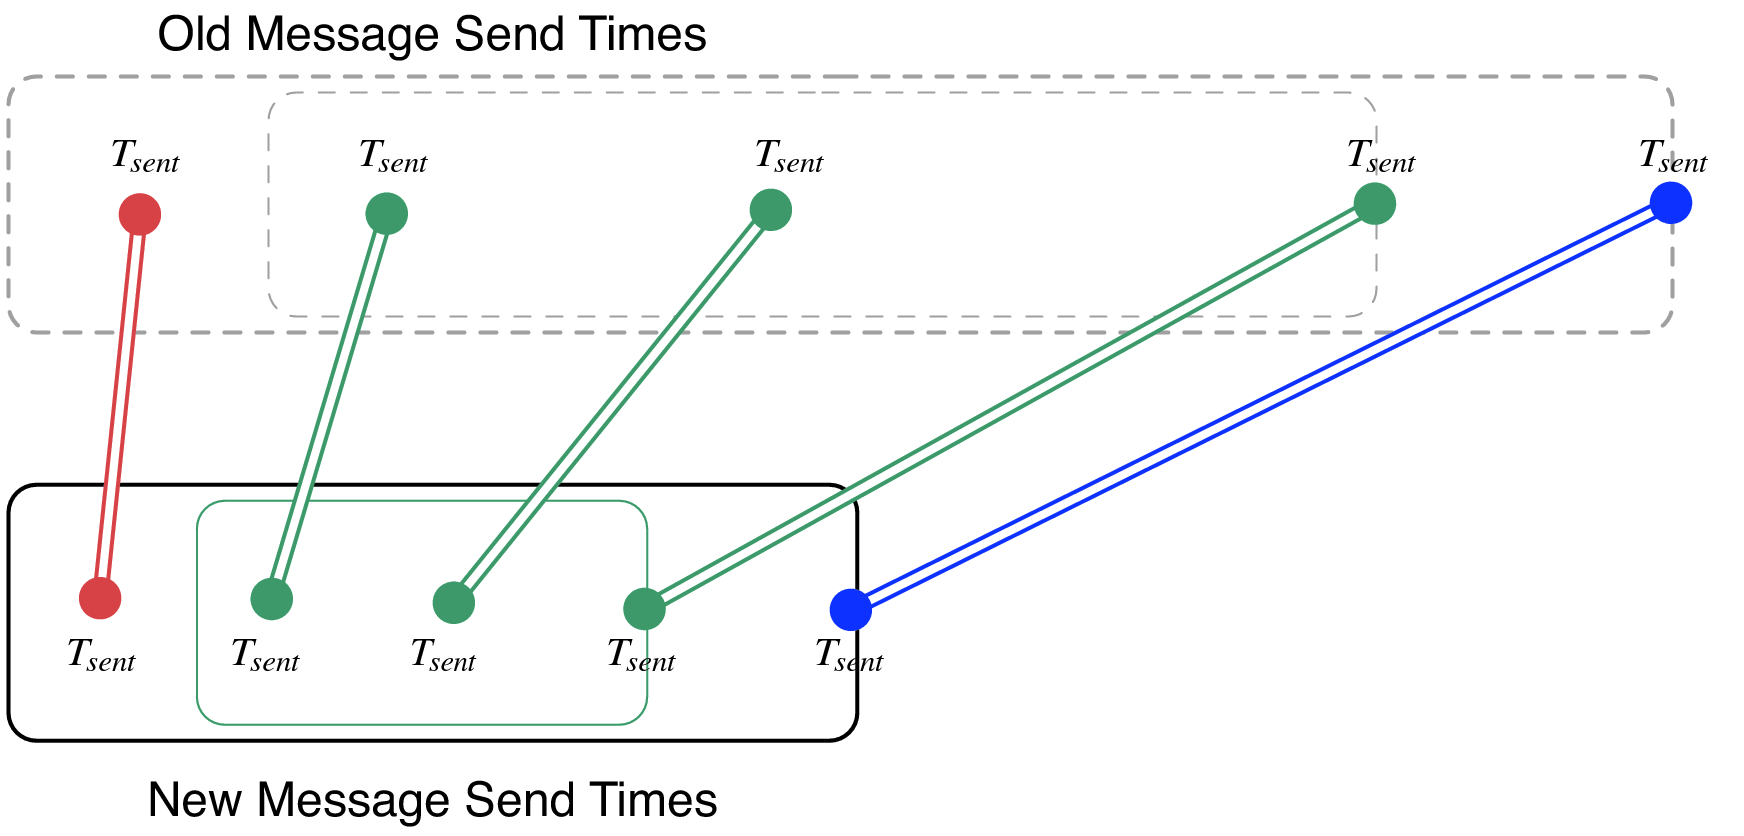
\includegraphics[width=6in]{figures/event_diagram2}
\caption{Message send times for messages sent from an SEB are remapped linearly onto the new time ranges for the 
SEB, region by region.
\label{event_diagram2}}
\end{figure}

The messages in the message list for each SEB must also have their $T_{sent}$ times rewritten. This is accomplished by linearly mapping the old $T_{sent}$ value from to the new range for the enclosing SEB region, as shown in Figure \ref{event_diagram2}. Any message sent during the first portion will be mapped linearly onto the new first portion of the SEB. The new message $T_{recv}$ times are ignored by BigSimulator, so they do not need to be modified.


\subsubsection{Supported performance models}
The interpolation tool supports three types of models, as described in this subsection.
% \ref{sec:model:scale}, \ref{sec:model:parameterization}, and \ref{sec:model:partial}. 
The more sophisticated models use the least-square curve fitting technique. 
The current implementation uses the Gnu Scientific Library(gsl) to perform the
least-square fit to the given data. The library provides both the coefficients and a $\chi^2$ measure of the closeness of the fit to the input data. 


%%%%%%%%%%%%%%%%%%%%%%%%%%%%%%%%%%%%%%%%%%%%%%%%%%%%
\paragraph{Model 1: Scaling SEB durations by a constant factor}
%\label{sec:model:scale}}

In simple cases, a sufficient approximation of the performance of a parallel application can be obtained
by simply scaling the SEB durations by a constant factor.
As an example, a user may know that a desired target machine has processors that will execute
each SEB twice as fast as on an existing machine.
The application is emulated on the existing machine and the observed SEB durations are scaled
by a factor of $2.0$. Although simple, this method may be sufficient in many cases. It becomes
unnecessary to use the \texttt{startTraceBigSim()} and  \texttt{endTraceBigSim()} calls.
The scaling factor is hard coded in the interpolation tool as \texttt{time\_dilation\_factor}.
It is used to scale all blocks unless a suitable advanced model has a better method for approximating the 
block's duration. It will always be used to scale any portions of blocks that are not bracketed with
the calls \texttt{startTraceBigSim()} and  \texttt{endTraceBigSim()}.

\paragraph{Model 2: Extrapolation based on user's parameterizations}
%\label{sec:model:parameterization}}

The user can simply insert the bracketing calls  \texttt{startTraceBigSim()} and
  \texttt{endTraceBigSim()} around the computational kernels to log the times taken for each kernel.
In practice, the duration of the SEB will likely depend upon the data distribution and access patterns
for the parallel application. Thus, the user must specify parameters likely to influence the SEB duration.
The parameters can include variables indicating number of loop iterations, number of calls to
computational kernels, or sizes of accessed portions of data arrays. A model is built to
approximate the duration of any SEB based upon its specified parameters.

As an example, NAMD uses a number of different types of objects. The \texttt{compute} objects will spend varying amounts of time depending upon the lengths of their associated atom lists. If an atom list is large, more interactions are computed and thus more computation is performed. 
% Now the method is described in the context of a simple hypothetical molecular dynamics application. 
Meanwhile, assume that a Charm++ entry method called \texttt{doWork(atomList)} is where the majority
of the work from an application occurs. The function computes forces on atoms of various types.
Different calls to the function will contain different numbers and types of atoms.
The source code for  \texttt{doWork(atomList)} will be modified by the user to  contain calls to
\texttt{startTraceBigSim()} at the entry and  \texttt{endTraceBigSim()} at the exit of the function.
The program will be run, and the resulting timed samples will be used to build a model. Assume the expected runtime of \texttt{doWork(atomList)} is quadratic in the \texttt{atomList} length and linear in the number of carbon atoms in the \texttt{atomList}. The \texttt{endTraceBigSim()}  call would be provided with a descriptive name and a set of parameters, such as \texttt{endTraceBigSim(``doWork()'', $p_1$,$p_2$)},  where parameter $p_1$ is the length of \texttt{atomList} and parameter $p_2$ is the number of carbon atoms in \texttt{atomList}.

The goal of using a model is to be able to predict the execution time of any arbitrary call to
\texttt{doWork()}, given its parameters. The application can be run on an existing processor
or parallel cluster for only a few timesteps with the modified \texttt{doWork()} method. 
This run will produce a list of \{$\left(p_1,p_2\right)\rightarrow duration$\} records. 
A least squares method is applied to fit a curve $f(p_1,p_2)=c_1+c_2 p_1+c_3 p_1^2 + c_4 p_2$  
approximating the durations of the records. The least square method minimizes the sum of the
squares of the difference between the function $f$ evaluated at each parameter set and the actual
timing observed at those parameters. The least square method is provided
 $\left(1.0,p_1,p_1^2,p_2,time\right)$ for each sample point and produces the coefficients $c_n$ in $f$. 
An arbitrary set of parameters (in the current implementation, up to twenty) can be input
to $f$ to produce an approximation of the runtime of \texttt{doWork()} even though the particular instance was never timed before. 

\paragraph{Model 3: Extrapolation of partial executions with cycle accurate simulations 
and user's parameterizations}
%\label{sec:model:partial}}

In this case, a cycle accurate simulator can be used to simulate a small fraction of all SEBs for a run
 of the application. The partial execution is used to build a model which applies to the whole execution.
Parameterizations can be used as 
% in section \ref{sec:model:parameterization}
previously described,
so that only some fraction of the SEBs will be run in the expensive cycle-accurate simulator. 
In NAMD, for example, a sufficient model can be built from  a random sample of 2\% of the cycle-accurate SEB durations from four timeloop iterations. 
